\chapter{La búsqueda del incendio, pieza por pieza}

\begin{enpocas}
Cómo quedó programado el planificador \cod{busqueda_incendio}: la máquina de estados, la ruta en serpentina, el seguimiento del relieve, la estimación y confirmación del foco, el aviso GPS y la evasión de obstáculos, con sus fórmulas y parámetros.
\end{enpocas}
\label{cap:autonomia}

\begin{lstlisting}[style=bash]
ros2 launch cuadrirotor_sim simulacion.launch.py vehiculo:=tarot650 mundo:=bosque_grande \
    controlador:=sta mision:=busqueda
\end{lstlisting}

Con \cod{mision:=busqueda} el \emph{launch} agrega el detector y el planificador
\cod{busqueda_incendio}, y pone al controlador en modo \cod{externa}: deja de generar su propia
referencia y sigue la consigna que publica el planificador en \cod{/cuadrirotor/consigna}
(\cod{trajectory_msgs/MultiDOFJointTrajectoryPoint}: posición, velocidad, aceleración y guiñada).
El planificador corre a 50~Hz y limita la velocidad (5~m/s horizontal, 3~m/s vertical) y la
aceleración (1.5~m/s$^2$) de la consigna.

\section{Máquina de estados}

\begin{figure}[H]
\centering
\begin{tikzpicture}[
  est/.style={draw,rounded corners,fill=#1,minimum width=2.6cm,minimum height=0.9cm,align=center,font=\small},
  est/.default=green!10,
  fl/.style={-{Stealth[length=2.2mm]},thick},
  et/.style={font=\scriptsize,align=center,fill=white,inner sep=1pt}]
  \node[est=black!5] (des) at (0,0) {despegue};
  \node[est] (pat) at (0,-2.8) {patrulla};
  \node[est] (hum) at (7,-2.8) {hacia\_humo};
  \node[est] (apr) at (0,-6.2) {aproximacion};
  \node[est=yellow!20] (ver) at (7,-6.2) {verificacion};
  \node[est] (bajo) at (0,-8.9) {descenso};
  \node[est=red!12] (orb) at (0,-11.4) {orbita\\+ aviso GPS};
  \draw[fl] (des) -- node[et,left]{altura de búsqueda\\alcanzada} (pat);
  \draw[fl] (pat) to[bend left=18] node[et,above]{humo en 3 imágenes seguidas} (hum);
  \draw[fl] (hum) to[bend left=18] node[et,below]{humo perdido 6 s} (pat);
  \draw[fl] (pat) -- node[et,left]{hay estimación\\del foco} (apr);
  \draw[fl] (hum) -- node[et,pos=0.62,above,sloped]{hay estimación} (apr);
  \draw[fl] (apr) to[bend right=18] node[et,below]{en el anillo y solo con humo} (ver);
  \draw[fl] (ver) to[bend right=18] node[et,above,pos=0.7]{ve las llamas} (apr);
  \draw[fl] (ver.east) -- ++(1.3,0) |- node[et,pos=0.25,right]{2 min sin\\ver llamas} ($(pat.north east)+(0,0.8)$) -- (pat.north east);
  \draw[fl] (apr) -- node[et,left]{en el anillo,\\estimación con llamas} (bajo);
  \draw[fl] (bajo) -- node[et,left]{altura de órbita\\y mirando al foco} (orb);
\end{tikzpicture}
\caption{Estados de \cod{busqueda_incendio}. En \emph{patrulla}, al terminar la ruta sin ver el
incendio, el dron la recorre de regreso y sigue vigilando.}
\label{fig:estados}
\end{figure}

\section{Ruta de barrido en serpentina}

La zona del bosque es el rectángulo $[-210,210]\times[-210,210]$~m. La ruta (\cod{cobertura.py},
\cod{ruta_serpentina}) avanza \textbf{hacia el frente del dron}: en el eje de la zona más parecido a
su rumbo al despegar (en la base mira a $+x$). Los barridos son perpendiculares al avance, de lado a
lado del bosque, separados $p\approx70$~m y a $p/2$ de los bordes; cada uno se une con el siguiente
por un semicírculo de radio $r = p/2 = 35$~m. Con $f$ la coordenada de avance, $l$ la lateral,
$\sigma=\pm1$ el lado de la vuelta y $\phi\in[0,\pi]$:
\begin{equation}
(f, l) = \big(f_k + r(1-\cos\phi),\ l_{fin} + \sigma r\sin\phi\big).
\end{equation}
La ruta se muestrea cada 5~m (2.6~km, $\approx$9~min a 5~m/s) y el dron persigue un punto 10~m
adelante sobre ella (\cod{anticipo_ruta}), así que no frena en las vueltas: a 5~m/s la vuelta pide
$v^2/r = 0.7$~m/s$^2$. La versión anterior (\cod{patron: franjas}) recorría franjas este-oeste con
vueltas en ángulo recto, deteniéndose en cada vértice.

\begin{figure}[H]
\centering
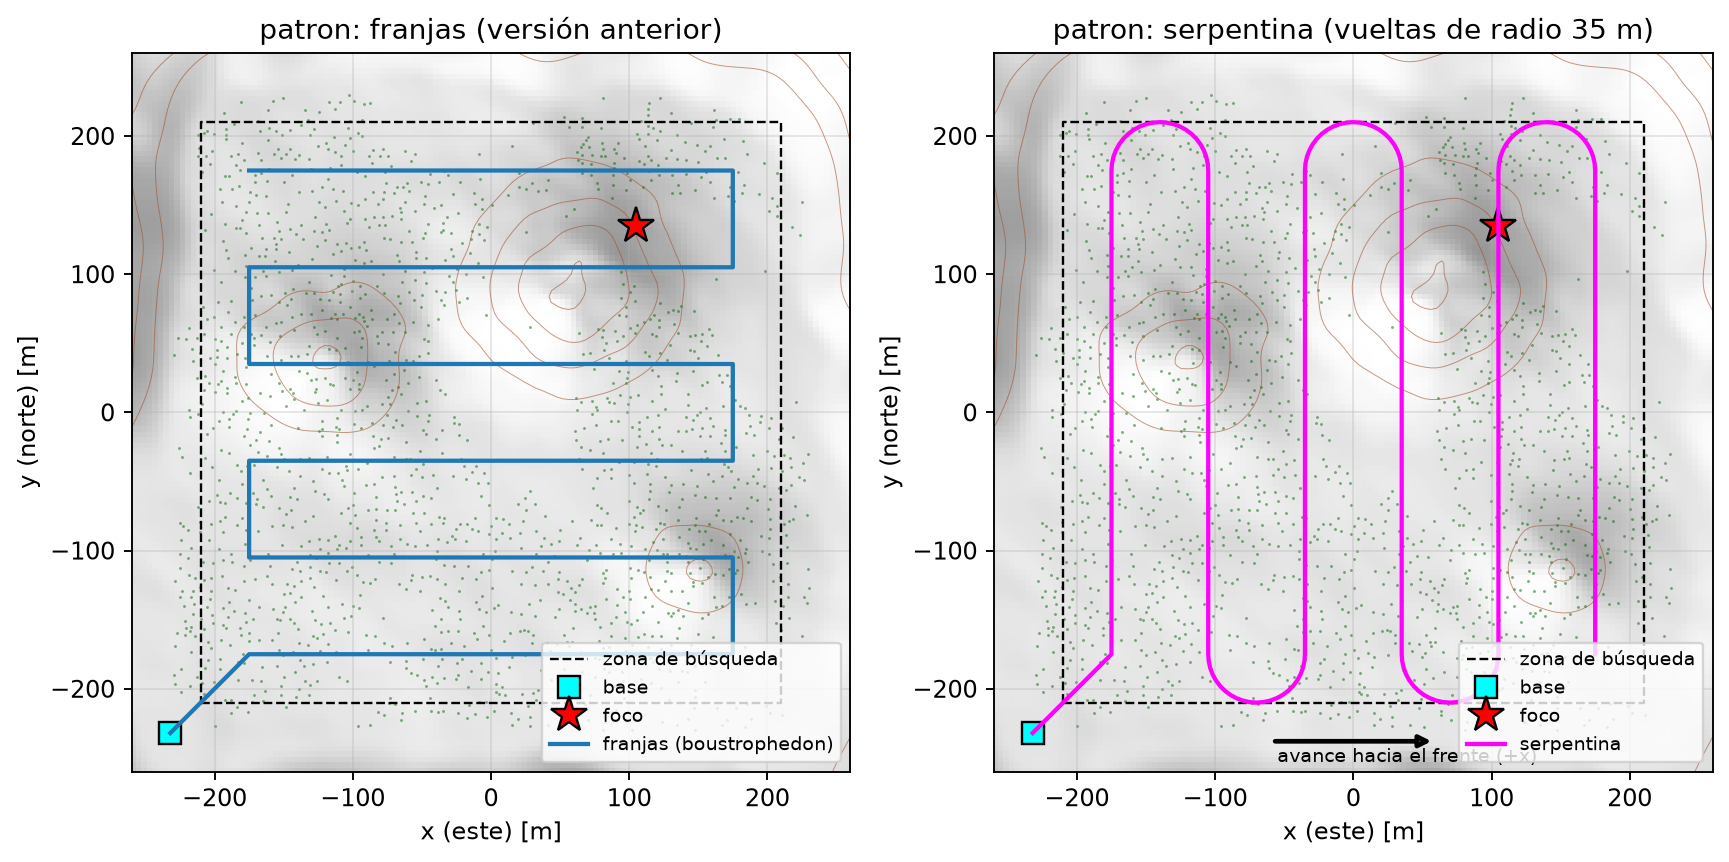
\includegraphics[width=\textwidth]{rutas.png}
\caption{Rutas sobre el relieve (curvas de nivel cada 10~m) y los árboles (puntos verdes).}
\label{fig:rutas}
\end{figure}

\section{Seguimiento del relieve}

Las alturas son \emph{sobre el suelo}. La altura de la consigna es
\begin{equation}
z = \max_{q\,\in\,[c,\ c + L\hat u]} h(q) + h_{busq},\qquad L = 50\ \text{m},\ h_{busq} = 30\ \text{m},
\end{equation}
el punto más alto del terreno entre la consigna $c$ y 50~m adelante (\cod{anticipacion}), más un
margen de 5~m a los lados. Así el dron empieza a subir antes de llegar a un cerro. El planificador
conoce el relieve (como un dron real con un mapa de elevación), pero no dónde está el incendio.

\section{Mapa de cobertura}

Cada 0.5~s se proyecta una rejilla de $24\times18$ rayos de la cámara sobre el relieve (hasta
150~m) y se marcan las celdas de $10\times10$~m que ya se vieron. Se publica el porcentaje en
\cod{/cuadrirotor/busqueda/cobertura} y el mapa en \cod{/cuadrirotor/busqueda/mapa_cobertura}
(\cod{nav_msgs/OccupancyGrid}, 0 = vista), junto con la ruta en \cod{/cuadrirotor/busqueda/ruta}.
Se ven en RViz con el marco \cod{world}.

\section{Estimación de la posición del foco}

Cada detección se empareja con la pose del dron en el instante de la imagen. El rayo de la cámara
por el centro de la caja $(u,v)$ es
\begin{equation}
d = R\,R_c\begin{bmatrix}1\\ -(u - W/2)/f\\ -(v - H/2)/f\end{bmatrix},\qquad
f = \frac{W/2}{\tan(\text{HFOV}/2)},
\end{equation}
con $R_c$ la inclinación de 30° de la cámara.

\textbf{Con llamas.} El rayo se corta con la superficie 1.1~m sobre el suelo (media altura de las
llamas) con \cod{Terreno.cortar_rayo}, solo si el corte queda a menos de 100~m
(\cod{alcance_llamas}). La estimación es la mediana de los últimos 15 cortes (con al menos 5).

\textbf{Con humo.} La columna es vertical sobre el foco, así que cada detección da solo un rumbo
$\hat n_i$ desde la posición $c_i$ de la cámara. Con rumbos desde puntos distintos (dispersión de
más de 0.25~rad) se busca el punto más cercano a todas las rectas por mínimos cuadrados:
\begin{equation}
\hat x = \Big(\sum_i P_i\Big)^{-1}\sum_i P_i\,c_i,\qquad P_i = I - \hat n_i\hat n_i^\top .
\end{equation}

\begin{leccion}
Antes del límite \cod{alcance_llamas}, con el foco en $(-150,60)$ la primera estimación caía en
$(-137,110)$: de lejos el rayo roza el suelo y un error pequeño en la caja da decenas de metros.
\end{leccion}

\section{Verificación: solo con llamas se confirma}

Si al llegar al anillo de órbita la estimación sigue saliendo solo del humo, el dron entra en
\emph{verificacion}: rodea el punto estimado a 35~m y a la altura de búsqueda, mirándolo, hasta ver
las llamas; con ellas vuelve a \emph{aproximacion} con la estimación corregida. Si no las ve en
2~min, descarta la estimación y sigue la patrulla. Solo con llamas baja a orbitar y avisa.

\section{Órbita}

Radio 14~m, $\omega = 0.12$~rad/s (con rampa de 4~s), cámara hacia el foco y altura
\begin{equation}
z_{orb} = \max\big(h(\text{foco}) + 18\ \text{m},\ \max_{\text{anillo}} h + 14\ \text{m}\big),
\end{equation}
por encima de las copas (los árboles miden hasta 8.2~m). Si el LiDAR ve algo más alto bajo el
anillo, sube (a lo más 1~m/s).

\begin{figure}[H]
\centering
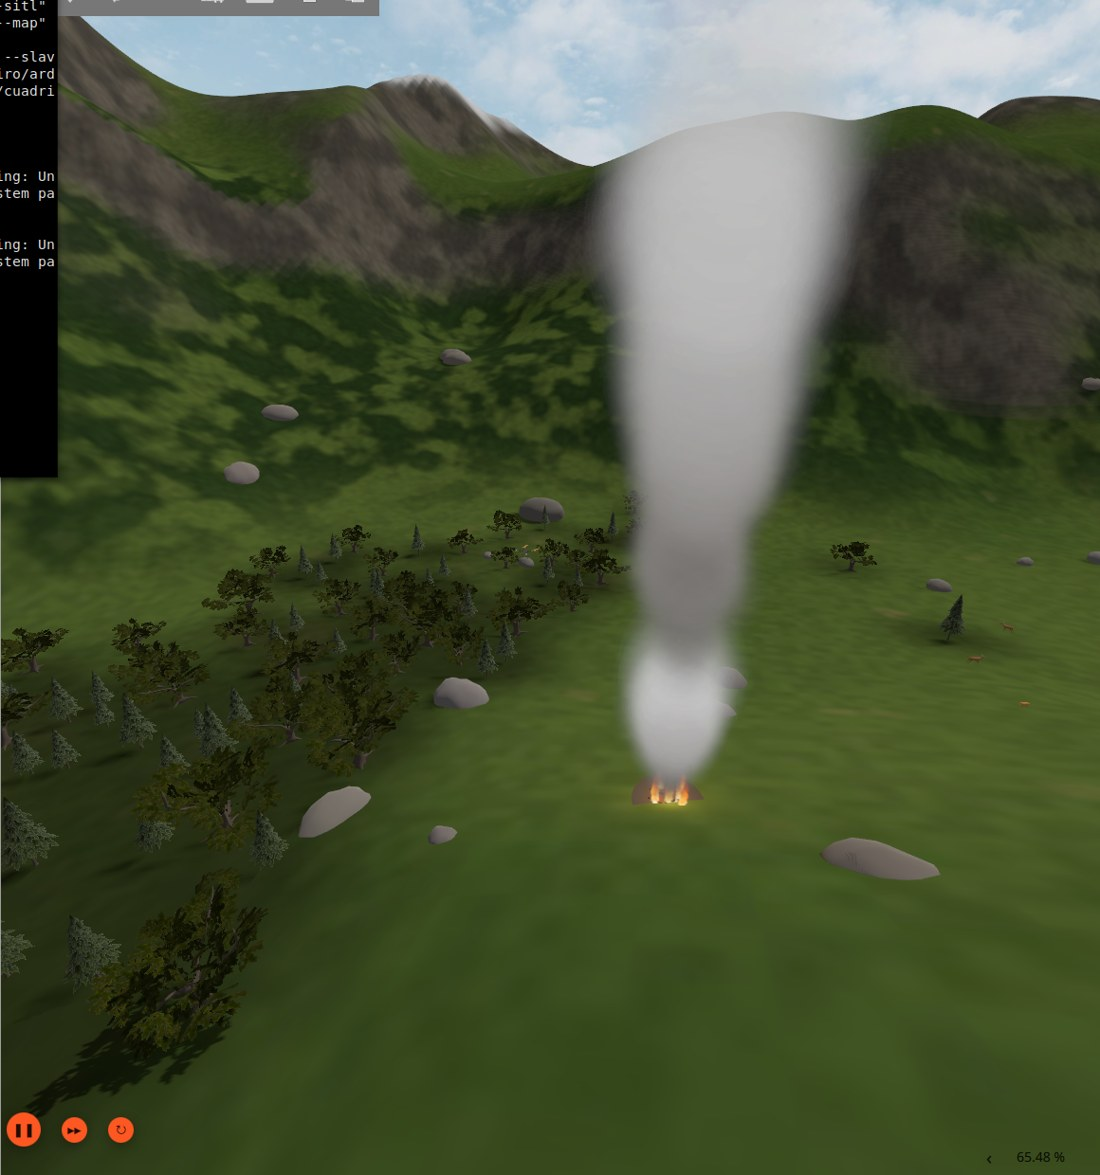
\includegraphics[width=0.62\textwidth]{gazebo_humo.jpg}
\caption{El dron llegando al foco: la cámara de Gazebo sigue al dron desde atrás.}
\end{figure}

\section{Aviso con las coordenadas GPS}
\label{sec:gps}

Al empezar la órbita (foco confirmado y visto de cerca) el planificador publica una sola vez:
\begin{itemize}
  \item \cod{/cuadrirotor/incendio/gps}: \cod{sensor_msgs/NavSatFix} con latitud, longitud, altitud
        y la dispersión de los cortes de las llamas como incertidumbre;
  \item \cod{/cuadrirotor/incendio/alerta}: el aviso de texto.
\end{itemize}
Los dos con QoS \emph{transient local}: quien se suscriba después también lo recibe. Además lo
escribe en la terminal y agrega una línea a \cod{~/incendios_detectados.csv}:

\begin{lstlisting}
INCENDIO CONFIRMADO 2026-10-23 04:26:47
  GPS: 19.294219, -99.310000  (19°17'39.2"N 99°18'36.0"W)
  Altitud del suelo: 3019 m   incertidumbre: ±1.0 m
  Mapa: https://www.google.com/maps?q=19.294219,-99.310000
  Local: (105.1, 135.0) m
\end{lstlisting}

Para recibirlo desde otra terminal: \cod{ros2 topic echo /cuadrirotor/incendio/alerta}.

\textbf{Conversión ENU $\rightarrow$ WGS84} (\cod{geo.py}). El origen del mundo se puso, como
supuesto, en el Parque Nacional Desierto de los Leones (CDMX), un bosque de oyamel con incendios
casi cada temporada seca: $\varphi_0 = 19.2930^\circ$, $\lambda_0 = -99.3110^\circ$, $h_0 = 3000$~m (el
relieve del mundo no es el real; parámetro \cod{origen_gps} para cambiarlo). La conversión es
exacta sobre el elipsoide WGS84 ($a = 6378137$~m, $e^2 = 6.69437999014\times10^{-3}$). El origen
pasa a ECEF con $N(\varphi) = a/\sqrt{1-e^2\sin^2\varphi}$:
\begin{equation}
X_0 = (N+h_0)\cos\varphi_0\cos\lambda_0,\quad
Y_0 = (N+h_0)\cos\varphi_0\sin\lambda_0,\quad
Z_0 = (N(1-e^2)+h_0)\sin\varphi_0 ,
\end{equation}
el punto $(x,y,z)$ en ENU se rota al ECEF,
\begin{equation}
\begin{bmatrix}X\\Y\\Z\end{bmatrix} = \begin{bmatrix}X_0\\Y_0\\Z_0\end{bmatrix} +
\begin{bmatrix}
-\sin\lambda_0 & -\sin\varphi_0\cos\lambda_0 & \cos\varphi_0\cos\lambda_0\\
\cos\lambda_0 & -\sin\varphi_0\sin\lambda_0 & \cos\varphi_0\sin\lambda_0\\
0 & \cos\varphi_0 & \sin\varphi_0
\end{bmatrix}
\begin{bmatrix}x\\y\\z\end{bmatrix},
\end{equation}
y se regresa a geodésicas iterando $\varphi \leftarrow \operatorname{atan2}\big(Z,\ p(1 - e^2N/(N+h))\big)$,
$h = p/\cos\varphi - N$, con $p = \sqrt{X^2+Y^2}$ y $\lambda = \operatorname{atan2}(Y, X)$.

\section{Evasión de obstáculos}

Se pidió que el dron no choque con las montañas ni con los árboles. Toda consigna, salvo la de la
órbita, pasa por dos filtros (\cod{_seguro} del planificador y \cod{cuadrirotor_sim/evasion.py}):

\subsection{Relieve: primero subir}

Con \cod{altura_seguridad} $> 0$ (10~m en el mundo grande), si la consigna está a menos de esa
altura sobre el punto más alto del terreno en los próximos 25~m, el objetivo horizontal se congela
en la posición actual y solo se sube. El dron nunca avanza ``hacia'' una ladera más rápido de lo
que puede subir.

\subsection{Árboles, rocas y animales: LiDAR y histograma polar}

\begin{enumerate}
  \item \textbf{Memoria de obstáculos.} Cada nube del LiDAR pasa al marco del mundo con la pose del
        dron en ese instante, $p_w = p + R\,(q + r_{lidar})$. Se quitan los puntos a menos de 1.5~m
        del DEM (son el suelo) y el resto se guarda en vóxeles de 1~m, olvidando lo que queda a más
        de 60~m del dron. Se publican en \cod{/cuadrirotor/evasion/obstaculos}.
  \item \textbf{¿Está libre el camino?} Se toman los puntos a la altura del dron ($\pm3$~m) y a menos
        de 20~m. Si ninguno queda a menos de $r = 3$~m del tramo recto hacia el objetivo, la consigna
        no se toca.
  \item \textbf{Histograma polar} (como VFH). Si el tramo está bloqueado, se dividen las direcciones
        en 72 sectores de 5°. Un punto a distancia $d$ y ángulo $\theta$ bloquea los sectores dentro de
        $\theta\pm\big(\arcsin(r/d) + 2.5^\circ\big)$, es decir, todo rumbo que pasaría a menos de $r$ de él.
  \item \textbf{Elección.} Se toma el sector libre que minimiza
        $|\theta - \theta_{obj}| + 0.3\,|\theta - \theta_{prev}|$ (el segundo término evita
        oscilar) y el objetivo pasa a ser un punto a 8~m en esa dirección. Si todos están bloqueados,
        el objetivo es subir 4~m.
  \item \textbf{Histéresis.} Mientras está desviado, solo vuelve al tramo recto cuando queda libre con
        $1.4\,r$.
  \item \textbf{Al bajar} no entra a menos de $r$ de lo más alto que tenga debajo.
\end{enumerate}

\begin{figure}[H]
\centering
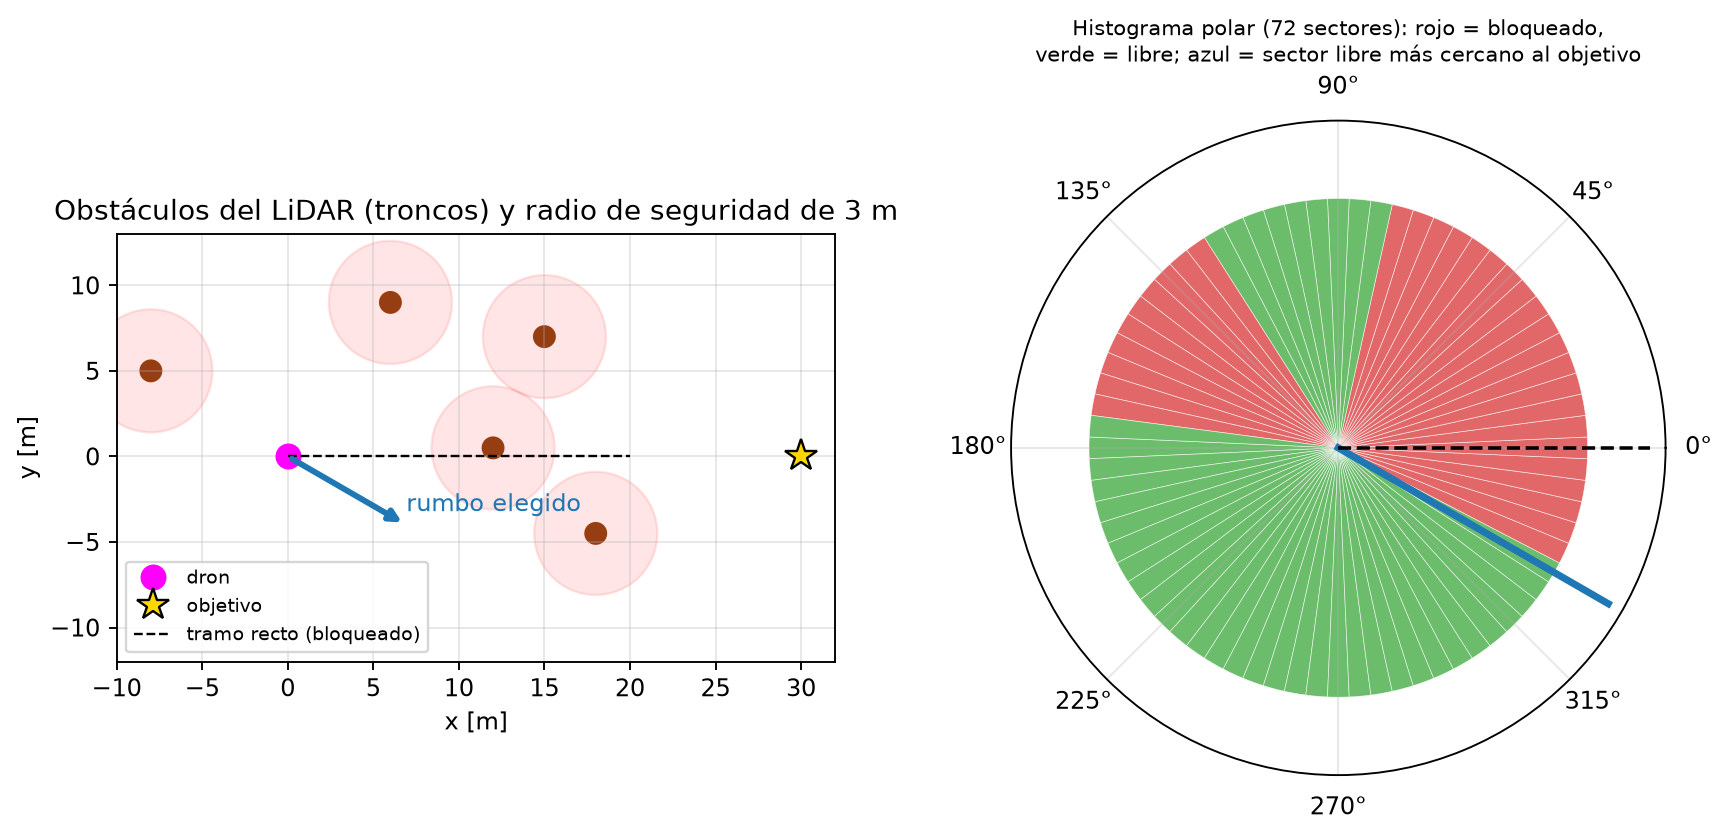
\includegraphics[width=\textwidth]{vfh.png}
\caption{Ejemplo del algoritmo: el tramo recto al objetivo choca con un tronco; el histograma polar
marca los sectores bloqueados y el dron toma el libre más cercano al rumbo del objetivo.}
\label{fig:vfh}
\end{figure}

El núcleo de \cod{Evasion.corregir}:
\begin{lstlisting}[style=py]
r = np.linalg.norm(Q, axis=1)                      # puntos (xy relativos) a la altura del dron
ang = np.arctan2(Q[:, 1], Q[:, 0])
ancho = np.arcsin(np.minimum(1.0, self.radio / np.maximum(r, 1e-3))) + self.medio_sector
bloq = (np.abs(envolver(self.th[:, None] - ang[None, :])) < ancho[None, :]).any(axis=1)
if bloq.all():                                     # sin salida: sube
    return np.array([c[0], c[1], c[2] + self.subida])
costo = np.abs(envolver(self.th - rumbo_g))
if self.rumbo_previo is not None:
    costo = costo + 0.3 * np.abs(envolver(self.th - self.rumbo_previo))
costo[bloq] = np.inf
rumbo = float(self.th[np.argmin(costo)])
\end{lstlisting}

\textbf{Prueba.} Para forzar la evasión se puso \cod{altura_busqueda: 5} (5~m sobre el suelo, entre
árboles de hasta 8.2~m). En 540~m de patrulla el dron se desvió 12 veces y \textbf{ninguna muestra
quedó dentro de una copa}: la holgura mínima a la copa más cercana fue de 0.5~m, a unos 2.2~m/s. A
los 30~m de la búsqueda normal los árboles no estorban y la evasión casi nunca actúa.

\begin{figure}[H]
\centering
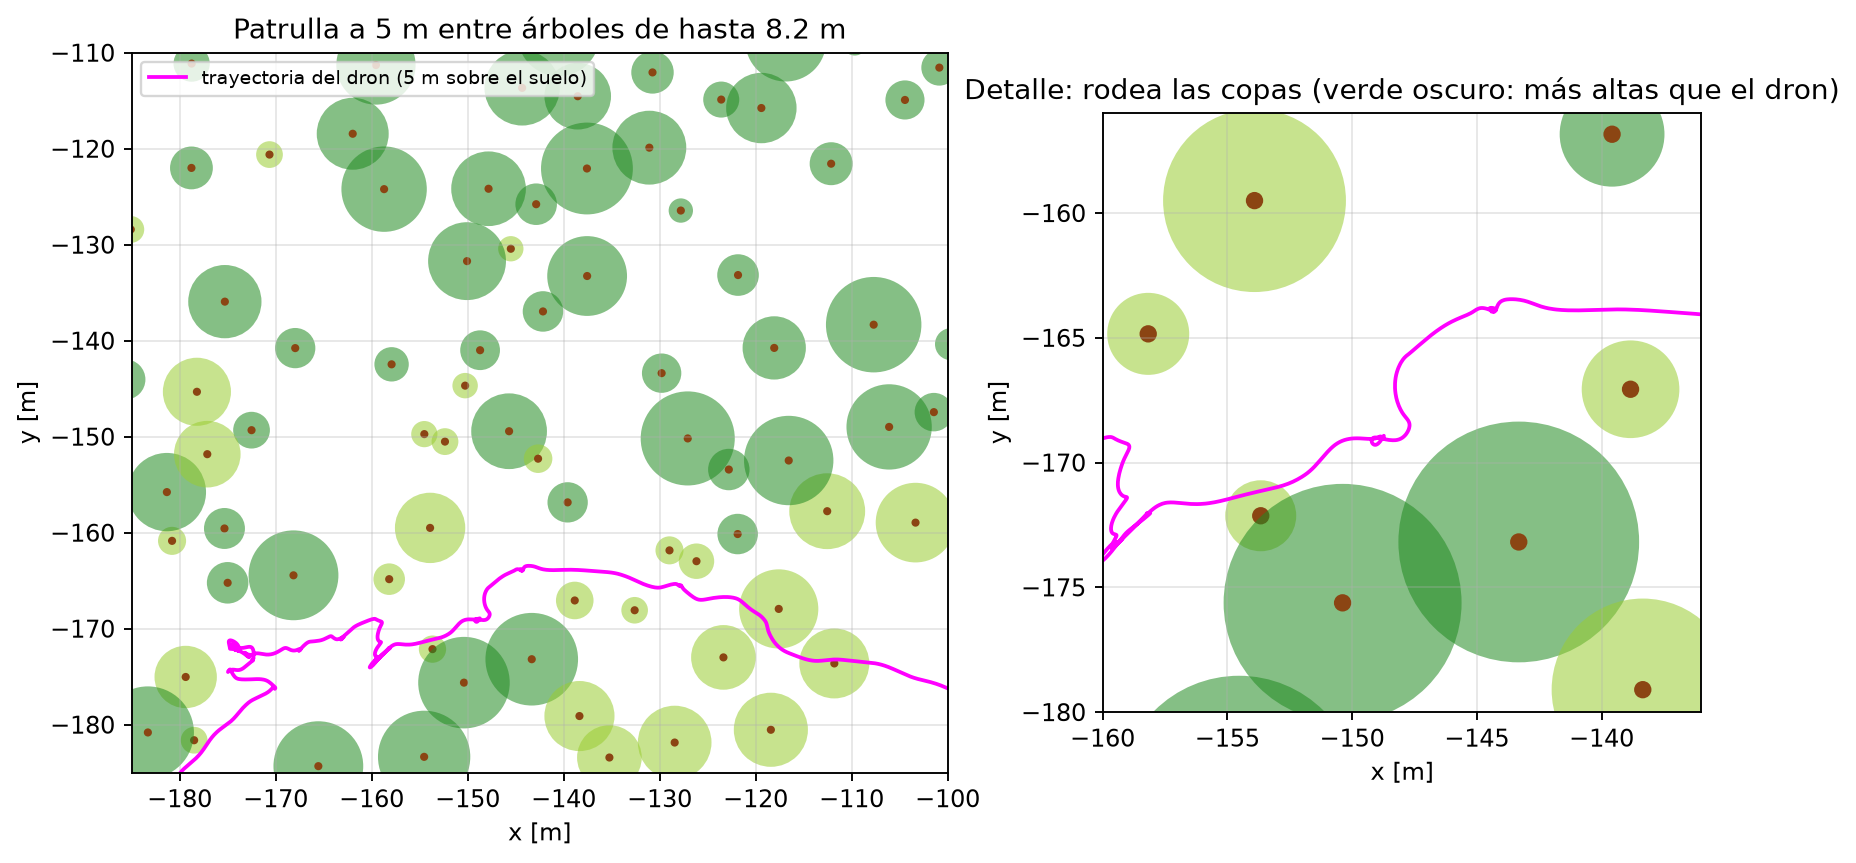
\includegraphics[width=\textwidth]{evasion_bajo.png}
\caption{Trayectoria real del dron (odometría de Gazebo) en la prueba a 5~m sobre el suelo. Los
círculos son las copas: verde oscuro, más altas que el dron.}
\end{figure}

\section{Parámetros del planificador}

\begin{longtable}{>{\raggedright\arraybackslash}p{4.3cm}>{\raggedright\arraybackslash}p{2.6cm}p{8.2cm}}
\toprule
\textbf{Parámetro} & \textbf{Valor} & \textbf{Significado} \\ \midrule \endhead
\cod{zona} & $[-210, 210]^2$ & rectángulo del bosque que se recorre [m] \\
\cod{patron} & serpentina & \cod{serpentina} o \cod{franjas} \\
\cod{separacion} & 70 & entre barridos [m] \\
\cod{anticipo_ruta} & 10 & distancia del punto que persigue sobre la ruta [m] \\
\cod{altura_busqueda} & 30 & sobre el suelo [m] \\
\cod{anticipacion} & 50 & mira el relieve esta distancia adelante [m] \\
\cod{velocidad}, \cod{velocidad_vertical} & 5, 3 & [m/s] \\
\cod{aceleracion} & 1.5 & [m/s$^2$] \\
\cod{alcance_vision} & 150 & para la cobertura [m] \\
\cod{alcance_llamas} & 100 & solo usa cortes de llamas más cercanos [m] \\
\cod{altura_orbita}, \cod{altura_minima_copas} & 18, 14 & órbita sobre el foco y sobre el anillo [m] \\
\cod{radio}, \cod{omega} & 14, 0.12 & órbita [m], [rad/s] \\
\cod{radio_verificacion}, \cod{tiempo_verificacion} & 35, 120 & [m], [s] \\
\cod{altura_seguridad} & 10 & sobre el relieve que tiene adelante [m] \\
\cod{radio_evasion}, \cod{alcance_evasion} & 3, 20 & [m] \\
\cod{evasion} & true & activa la evasión con el LiDAR \\
\cod{origen_gps} & (19.293, $-$99.311, 3000) & latitud, longitud y altitud del origen \\
\cod{registro_incendios} & \cod{~/incendios_detectados.csv} & CSV de avisos \\
\bottomrule
\end{longtable}
